\input{../YKY-preamble}

\title{Classical interpretation of the quantum state $\Psi$}
\author{\cc{甄景贤}{Yan King Yin} {\footnotesize general.intelligence@gmail.com}}

\begin{document}

	\setlength{\parindent}{0pt}
	\setlength{\parskip}{2.8ex plus0.8ex minus0.8ex}
	
	\maketitle
	
\begin{abstract}
	Taking $\Psi$ as the exponentiation of the classical action $S$, we find that Schr\"odinger's equation can be derived from the classical Hamilton-Jacobi equation.  This connection has already been considered by Schr\"odinger himself in one of his 1926 papers, but he dismissed it as ``incomprehensible''.  We propose that this interpretation is actually valid, and that quantum mechanics is compatible with classical mechanics.
\end{abstract}

Recently I seem to have ``discovered'' a way to interpret the classical-quantum correspondence.  This insight is already contained in many textbooks, though perhaps not everyone recognizes its physical / philosophical significance.  Previously, the transition from classical to quantum mechanics has always been \textit{heuristical}, rather than mathematically precise.

Compare the classical and quantum equations:
\begin{eqnarray}
\boxed{\mbox{CLASSICAL: Hamilton-Jacobi}} \quad
\frac{\partial S}{\partial t} = - H
\label{Hamilton-Jacobi-eqn2}
\\
\boxed{\mbox{QUANTUM: Schr\"{o}dinger}} \quad
i \hbar \frac{\partial \Psi}{\partial t} = \hat{H} \Psi .
\label{Schrodinger-eqn}
\end{eqnarray}

The 2 equations can be made \textit{identical} by introducing $\Psi$ as the \textbf{exponentiation} of $S$:
\begin{equation}
\boxed{\mbox{exponentiation ansatz}} \quad
\Psi = e^{i S /\hbar}
\label{eqn-exponentiation}
\end{equation}

Assuming that the Hamilton-Jacobi equation (\ref{Hamilton-Jacobi-eqn2}) holds for a \textit{classical} system, the substitution of the exponeniation formula (\ref{eqn-exponentiation}) results in the following equation:
\begin{equation}
\begin{tikzcd}[column sep = 7em]
\frac{\partial S}{\partial t} = - H \quad
\arrow[Rightarrow, r, "$\Psi = \exp \{ i S / \hbar \} $", align=center]
& \quad i \hbar \frac{\partial \Psi}{\partial t} = H \Psi .
\end{tikzcd}
\end{equation} 
which looks very similar to Sch\"odinger's equation, except that $H$ still looks different from $\hat{H}$.

\section{Momentum operator}
\label{sec:momentum-operator}

To show that $H = \hat{H}$ (under our exponentiation ansatz (\ref{eqn-exponentiation})), it suffices to show that the quantum momentum operator $\hat{p}$ obeys:
\begin{equation}
\hat{p} \; \Psi \equiv -i \hbar \nabla \Psi \equiv - i \hbar \frac{\partial}{\partial x} \Psi \stackrel{?}{=} p \; \Psi
\label{eqn:momentum-operator}
\end{equation}
where $p$ is the classical momentum.

Note that (\ref{eqn:momentum-operator}) is a \textbf{postulate} of quantum mechanics and used to be regarded as an article of \textit{faith}.

The derivation below uses only classical equalities:
\begin{eqnarray}
\hat{p} \; \Psi = -i \hbar \frac{\partial}{\partial x} \Psi
&=&  -i \hbar \frac{\partial}{\partial x} e^{i S / \hbar} \nonumber \\
&=& -i \hbar \; e^{i S / \hbar} \frac{i}{\hbar} \frac{\partial S}{\partial x} \nonumber \\
&=& \frac{\partial S}{\partial x} \Psi \nonumber \\
&=& \frac{\partial \int L dt}{\partial x} \Psi \nonumber \\
&=& \int \frac{\partial L}{\partial x} dt \; \Psi \nonumber \\
&=& \int \frac{d}{dt} \left( \frac{\partial L}{\partial \dot{x}} \right) dt \; \Psi \nonumber \\
&=& \frac{\partial L}{\partial \dot{x}} \; \Psi \nonumber \\
&=& p \; \Psi
\end{eqnarray}
where we have made use of the \textbf{Euler-Lagrange equation}:
\begin{equation}
\frac{d}{dt} \left( \frac{\partial L}{\partial \dot{x}} \right) - \frac{\partial L}{\partial x} = 0
\end{equation}
and the classical definition of the action $S$ as:
\begin{equation}
S = \int L \; dt
\end{equation}
and the definition of the \textbf{conjugate momentum} in Hamiltonian mechanics:
\begin{equation}
p := \frac{\partial L}{\partial \dot{x}} .
\end{equation}
The latter can be easily seen to be true for the classical linear momentum $p = m \dot{x}$ and with $L = \frac{1}{2} m \dot{x}^2$.

\section{Energy operator}
\label{sec:energy-operator}

Let's try the energy operator using the same technique as above:
\begin{equation}
\hat{E} = - \frac{\hbar^2}{2 m} \Delta \equiv - \frac{\hbar^2}{2 m} \frac{\partial^2}{\partial x^2} .
\end{equation}

\begin{eqnarray}
\hat{E} \; \Psi = - \frac{\hbar^2}{2 m} \Delta \Psi
&=& - \frac{\hbar^2}{2 m} \frac{\partial^2}{\partial x^2} e^{i S / \hbar} \nonumber \\
&=& - \frac{\hbar^2}{2 m} \left[ \frac{\partial}{\partial x} \left( e^{i S / \hbar} \cdot \frac{\partial S}{\partial x} \cdot \frac{i}{\hbar} \right)  \right] \nonumber \\
&=& - \frac{i \hbar}{2 m} \left[ \frac{\partial}{\partial x} e^{i S / \hbar} \cdot \frac{\partial S}{\partial x}  + e^{i S / \hbar} \cdot \frac{\partial^2 S}{\partial x^2} \right] \nonumber \\
&=& - \frac{i \hbar}{2 m} \left[ \frac{i}{\hbar} \cdot e^{i S / \hbar} \cdot \left( \frac{\partial S}{\partial x} \right)^2  + e^{i S / \hbar} \cdot \frac{\partial^2 S}{\partial x^2} \right] \nonumber \\
&=& - \frac{i \hbar}{2 m} \Psi \left[ \frac{i}{\hbar} \left( \frac{\partial \int L dt}{\partial x} \right)^2  + \frac{\partial^2 \int L dt}{\partial x^2} \right] \nonumber \\
&=& - \frac{i \hbar}{2 m} \Psi \left[ \frac{i}{\hbar} \left( \int \frac{\partial L}{\partial x} dt \right)^2  + \frac{\partial}{\partial x} \left( \int \frac{\partial L}{\partial x} dt \right) \right] \nonumber \\
&=& - \frac{i \hbar}{2 m} \Psi \left[ \frac{i}{\hbar} \left( \int \frac{d}{dt} \frac{\partial L}{\partial \dot{x}} dt \right)^2  + \frac{\partial}{\partial x} \left( \int \frac{d}{dt} \frac{\partial L}{\partial \dot{x}} dt \right) \right] \nonumber \\
&=& - \frac{i \hbar}{2 m} \Psi \left[ \frac{i}{\hbar} \left( \frac{\partial L}{\partial \dot{x}} \right)^2  + \frac{\partial}{\partial x} \left( \frac{\partial L}{\partial \dot{x}} \right) \right] \nonumber \\
&=& - \frac{i \hbar}{2 m} \Psi \left[ \frac{i}{\hbar} p^2  + \frac{\partial p}{\partial x} \right] \nonumber \\
&=& - \frac{i \hbar}{2 m} \Psi \left[ \frac{i}{\hbar} p^2  + 0 \right] \nonumber \\
&=& \frac{p^2}{2 m} \Psi \nonumber \\
&=& E \; \Psi
\end{eqnarray}

This does not look like coincidence.

\section{Relation to Feynman's path integral}

The exponentiation idea (\ref{eqn-exponentiation}) is already borne out by Feynman's \textbf{path integral} formulation:  $S$ is the classical action which is a sum of infinitesimal elements, and the exponentiation causes it to become a product, hence the \textbf{Trotter product formula}.

\subsubsection{The propagator of $\Psi$}

It has been known that the time-evolution of $\Psi$ can be described by the \textbf{propagator} $U(t)$:
\begin{equation}
\Psi_t = U(t) \Psi_0 = e^{-i H t / \hbar} \; \Psi_0 .
\end{equation}
From the perspective of our new idea, the propagator is expressed this way precisely because the time-evolution of the action $S$ is governed by:
\begin{equation}
S_t = S_0 - H \Delta t
\end{equation}
where $H$ is the classical Hamiltonian.  So it all makes sense.

In Feynman's thesis (circa 1942), he only observed the time-propagator of $\Psi$ without identifying $\Psi$ with $\exp S$:
\begin{equation}
\vcenter{\hbox{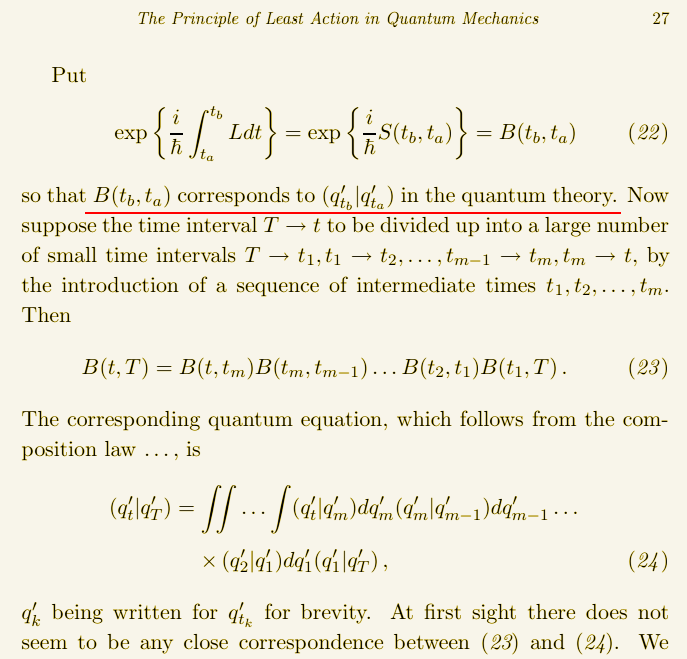
\includegraphics[scale=0.5]{Feynman-thesis-1.png}}} \nonumber
\end{equation}

Later in the same thesis, Feynman derived Schr\"odinger's equation from the classical harmonic oscillator, using the variational technique:
\begin{equation}
\vcenter{\hbox{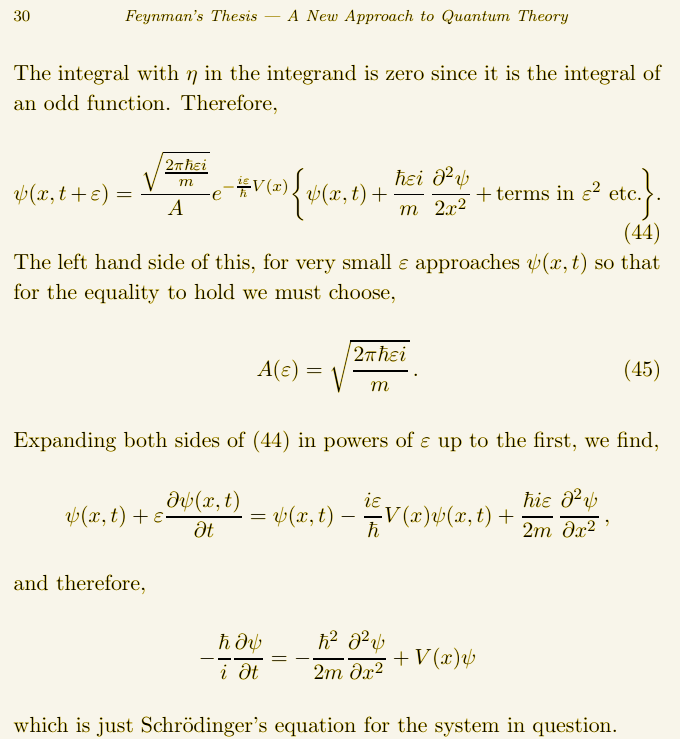
\includegraphics[scale=0.5]{Feynman-thesis-2.png}}} \nonumber
\end{equation}
but he seems unaware, at least around 1942, of the possibility of using (\ref{eqn-exponentiation}) directly.

Also, in Dirac's 1932 paper, \textit{The Lagrangian in Quantum Mechanics}, he also mentioned the propagator without equating $\Psi$ with the exponentiated action:
\begin{equation}
\vcenter{\hbox{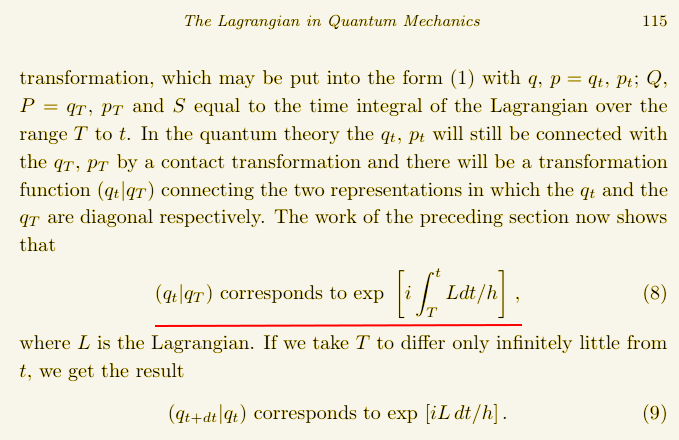
\includegraphics[scale=0.5]{Dirac-1932.png}}} \nonumber
\end{equation}

\section{Switching between $\Psi$ and $S$}

Indeed, in 1926 Schr\"odinger \parencite{Schrodinger1926} has already considered:
\begin{equation}
S = \hbar \ln \Psi
\end{equation}
with $\Psi$ a real function, but he dismissed this formula as ``incomprehensible'' (\textit{unverst\"andlich}).

I think we can understand the exponentiation of (\ref{eqn-exponentiation}) as transforming the classical action, which is an \textit{additive} quantity, into a \textit{multiplicative} quantity.  This is a purely mathematical construct.

The significance is that, after such a transformation, the quantum Schrodinger equation can be exactly identified with its classical counterpart, Hamilton-Jacobi equation.

In other words, if there is a classical action $S$ satisfying the Hamilton-Jacobi equation, then there would be a function $\Psi$ satisfying the Schr\"odinger equation.  However, the inverse function of (\ref{eqn-exponentiation}) is not unique.

Recall that a complex number, of unit length, in polar form is $e^{i \theta} = \cos \theta + i \sin \theta$.  So if $\Psi = e^{i S / \hbar}$ this means that $| \Psi |$ is automatically \textbf{normalized} to 1.  Moreover, $S$ behaves like a phase ``angle'' that causes $\Psi$ to \textbf{rotate} in the complex plane.  Also $\hbar = h / 2 \pi$, so the interpretation of $S / \hbar$ is that the Planck constant is the \textit{unit} upon which $S$ causes $\Psi$ to rotate;  in other words, $h$ is the \textit{quantum}.

The upshot is that the inverse function $S = - i \hbar \log \Psi$ will always yield a \textbf{real} value $\in \mathbb{R}$.  Thus the corresponding Hamilton-Jacobi equation is always valid.

\section{Probabilistic interpretation?}

In the Copenhagen interpretation, $\Psi$ is regarded as the quantum ``state'', and as the ``complex probability amplitude'' which yields the real probability via:
\begin{equation}
\mathbb{E} [ x ]
= \langle x \rangle
= \int dx \; | \Psi(x, t) |^2 .
\end{equation}
How might we re-interpret this interpretation in the new light?

\section{How does quantization arise?}

We have shown that the classical Hamilton-Jacobi equation leads to the \textbf{time-dependent} Schr\"odinger equation under the exponentiation ansatz.  We can then derive the \textbf{time-indepen\allowbreak dent} Schr\"odinger equation by making use of Bohr's concept of stationary states with well-defined energies. A stationary state has an energy $E$ and consequently a well-defined frequency $\nu = E / h$.  Its wave function $\Phi (x, y, z, t)$ may therefore be decomposed into 2 components:
\begin{equation}
\Phi (x, y, z, t) = \Psi (x, y, z) \cdot e^{-i E t / \hbar}
\end{equation}
of which the first component depends only on position.  From this we get the \textbf{time-indepen\allowbreak dent} Schrodinger equation:
\begin{equation}
\hat{H} \; \Psi = E \; \Psi .
\label{time-independent-Schrodinger}
\end{equation}

The solutions of the time-independent Schrödinger equation contain energy $E$ as a parameter. Some solutions are unacceptable from a physical point of view, because they diverge to $\infty$ as $x \rightarrow \infty$;  This is what leads to \textbf{quantization}.  Acceptable solutions are obtained only for specific discrete values of the energy parameter $E$ that are known as the eigen-values $E_n$ of the equation.  These eigen-values correspond to the stationary states that had been proposed by Bohr.

Such stationary states are intriguing because their probability density $\rho = | \Psi(\vect{r}, t) |^2 $ and all other probabilities are \textbf{constant} in time.

The paradigmatic example of quantization is the \textbf{harmonic oscillator}, with classical Hamiltonian defined as:
\begin{equation}
H = \frac{p^2}{2 m} + \frac{1}{2} k x^2
\label{harmonic-Hamiltonian}
\end{equation}
and the quantum-operator version defined similarly.

First, we start from the time-independent Schr\"odinger equation (\ref{time-independent-Schrodinger}) and try to solve it directly.  There are several methods.  One method is to set up a power series expansion which leads to recursive relations between the coefficients and \textbf{Kummer functions}.  Another, more abstract method is to introduce the \textbf{creation} and \textbf{annihilation} operators.  Both methods result in the discretization of energy levels.

But what if we try to solve (\ref{time-independent-Schrodinger}) by converting it back to the classical form, using the tricks of \S\ref{sec:momentum-operator} and \S\ref{sec:energy-operator}?  We end up getting back the Hamiltonian as the sum of kenetic energy and potential energy:
\begin{equation}
H = E = T + V
\end{equation}
as if we have done nothing.  This implies that we are merely dealing with a classical system whose Hamiltonian is given by (\ref{harmonic-Hamiltonian}).  We know that this is the Hamiltonian of a point mass under a simple quadratic potential, but it could also be describing \textit{other} systems whose Hamiltonian is same as the point mass, perhaps, with the mass distributed in space.

In the quantum version (\ref{time-independent-Schrodinger}), we assumed that $\Psi$ is a function in Hilbert space, which must not diverge to $\infty$ along the space axis.  This \textit{forces} $\Psi$ to take on certain shapes, namely the \textbf{eigen-functions}.  But this does not contradict the constraints of the classical equations.

If we take the inverse $S = - i \hbar \log \Psi$ we get back the classical action $S$ which may not be oscillatory.  This $S$ would be a spatial function compatible with the classical Lagrangian $L = T - V$.  

\section{Relation to the Bell inequality?}

Much of what we call ``quantum weirdness'' is abstracted by the Bell inequality.  Can one derive the Bell inequality from the Schr\"odinger equation?  Or, the Bell inequality depends also on the axioms of quantum mechanics?  This is an interesting question....

\section{Conclusion}

Quantum mechanics does \textit{not} contradict classical mechanics.  Quantum mechanical equations can be reduced to classical equations, the latter describe systems that are compatible with classical quantities such as the Hamiltonian $H$, Lagrangian $L$, and action $S$.  However, they do not tell us how the mass in question is distributed in space, or how the quantum waves are actually constituted as matter waves.

\begin{minipage}{0.15\textwidth}
	\begin{center}
		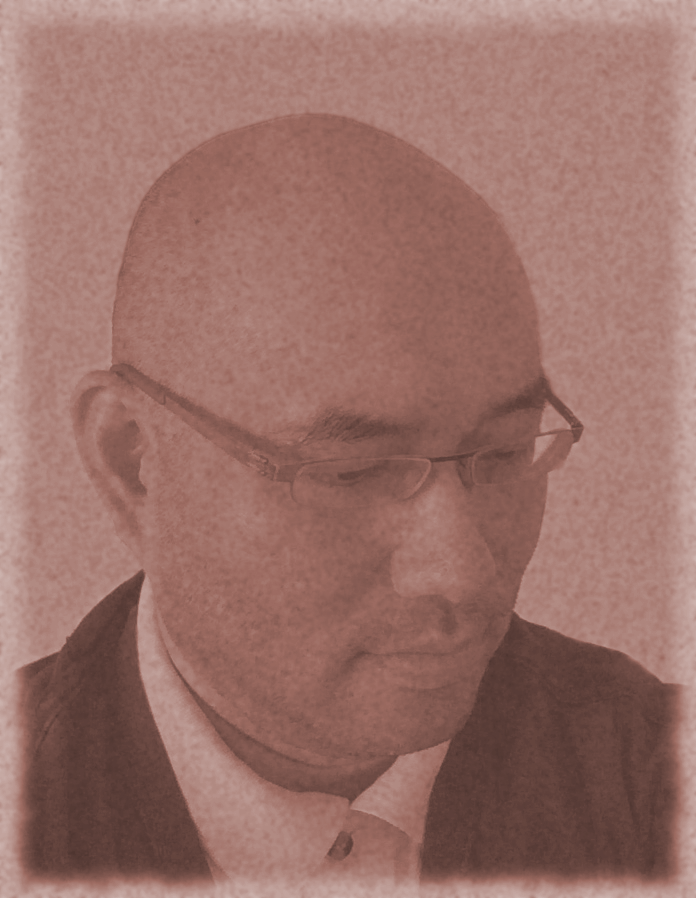
\includegraphics[scale=0.1]{../John_Grothendieck.png}
	\end{center}
\end{minipage}
\begin{minipage}{0.6\textwidth}
YKY is an independent researcher from Hong Kong.  His main focus is on AGI (artificial general intelligence).  Through his research in AI, he came into contact with the Hamilton-Jacobi-Bellman equation, which describes dynamic programming (reinforcement learning).  He has a long-time, though amateur, interest in the foundations of quantum mechanics.
\end{minipage}%

\nocite{Faria2010}
\nocite{Mann2018}
\nocite{Baaquie2014}
\nocite{Gustafson2003}
\nocite{Esposito2004}
\nocite{Cook1989}
\nocite{Gosson2017}
\nocite{Liberzon2012}
\nocite{Mueller-Kirsten2006}
\nocite{Merzbacher1998}
\nocite{Hameka2004}

\printbibliography

\end{document}